
\section{Điều chế và giải điều chế ASK (Amplitude Shift Keying)}
\label{section:1}
\subsection{Không gian tín hiệu 2-ASK:}
\label{subsection:1.1}
ASK (Binary Amplitude Shift Keying) là một loại kỹ thuật điều chế biên độ số. Tín hiệu ASK có dạng sóng giao động tần số f, sóng tín hiệu truyền đi được tạo ra bằng cách thay đổi biên độ của sóng mang.\\

\begin{center}
    \begin{figure}[htp]
    \begin{center}
     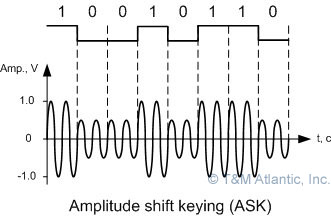
\includegraphics[]{Img/keying_ASK}
    \end{center}
    \label{refhinh1}
    \end{figure}
\end{center}

Trong điều chế 2-ASK, một bit sẽ được gán với một sóng mang với biên độ khác nhau.\\
Không gian tín hiệu 2-ASK:
\begin{center}
\begin{equation*}
   $ M = \{s_{1} = A_{1}sin(2\pi ft) ; s_{2} = A_{2}sin(2\pi ft)\} $
\end{equation*}
\end{center}
Cơ sở trực chuẩn: $b(t) = \sqrt{\frac{2}{T}}sin(2\pi ft)$ với $T = \frac{1}{R_{b}}$.
\subsection{Kênh tạp âm trắng có tính cộng AWGN}
Ở mọi hệ thống truyền thông, tín hiệu nhận được đều bị méo đi do có nhiễu. Ở đây, ta giả thiết nhiễu là nhiễu Gauss trắng có tính cộng. \\
Kênh AWGN có các tính chất sau:
\begin{itemize}
    \item Tuyến tính và bất biến theo thời gian
    \item Đáp ứng tần số lý tưởng $H(f) = 1$
    \item Tạp âm Gaus có tính cộng 
    \begin{itemize}
        \item Tiến trình ngẫu nhiên ergodic: các đặc trưng thống kê của tiến trình có thể suy ra được từ một chuỗi các mẫu đủ dài của nó
        \item Mỗi biến ngẫu nhiên tuân theo phân phối chuẩn Gauss với giá trị trung bình bằng 0
    \end{itemize}
    \item Mật độ công suất phổ tín hiệu là hằng số $G_{n}(f) = \frac{N_{0}}{2}$
    
\end{itemize}

\subsection{Bộ lọc phối hợp (Matched Filter)}
Chọn bộ lọc có đáp ứng xung $h(t) = b(T-t)$ ta được bộ lọc phối hợp.\\
Tín hiệu đầu vào bộ lọc là tín hiệu nhận được bên bộ thu: $\rho (t)$. \\
Đáp ứng xung là: $h(t) = b_{j}(t)$ \\
Đầu ra của bộ lọc phối hợp là: 
\begin{center}
    $y(t) = \int_{-\infty}^{+\infty} \rho(\tau)h(t-\tau)\  dx = \int_{-\infty}^{+\infty} \rho(\tau)b_{j}(T-t+\tau)\  dt$
\end{center}
Giả thiết lấy mẫu tín hiệu đầu ra tại thời điểm $T = 1$:
\begin{center}
    $y(t=T) = \int_{-\infty}^{+\infty} \rho(\tau)b_{j}(\tau)\  dx = \int_{0}^{T} \rho(\tau)b_{j}(\tau)\  d\tau$
\end{center}
Như vậy, sử dụng MF cho ta một phương án thay thế có thể được dùng để tính toán các phép chiếu $b_{j}(t)$ thay vì phải sử dụng các bộ tích phân các bộ tích phân
\begin{center}
    \begin{figure}[htp]
    \begin{center}
     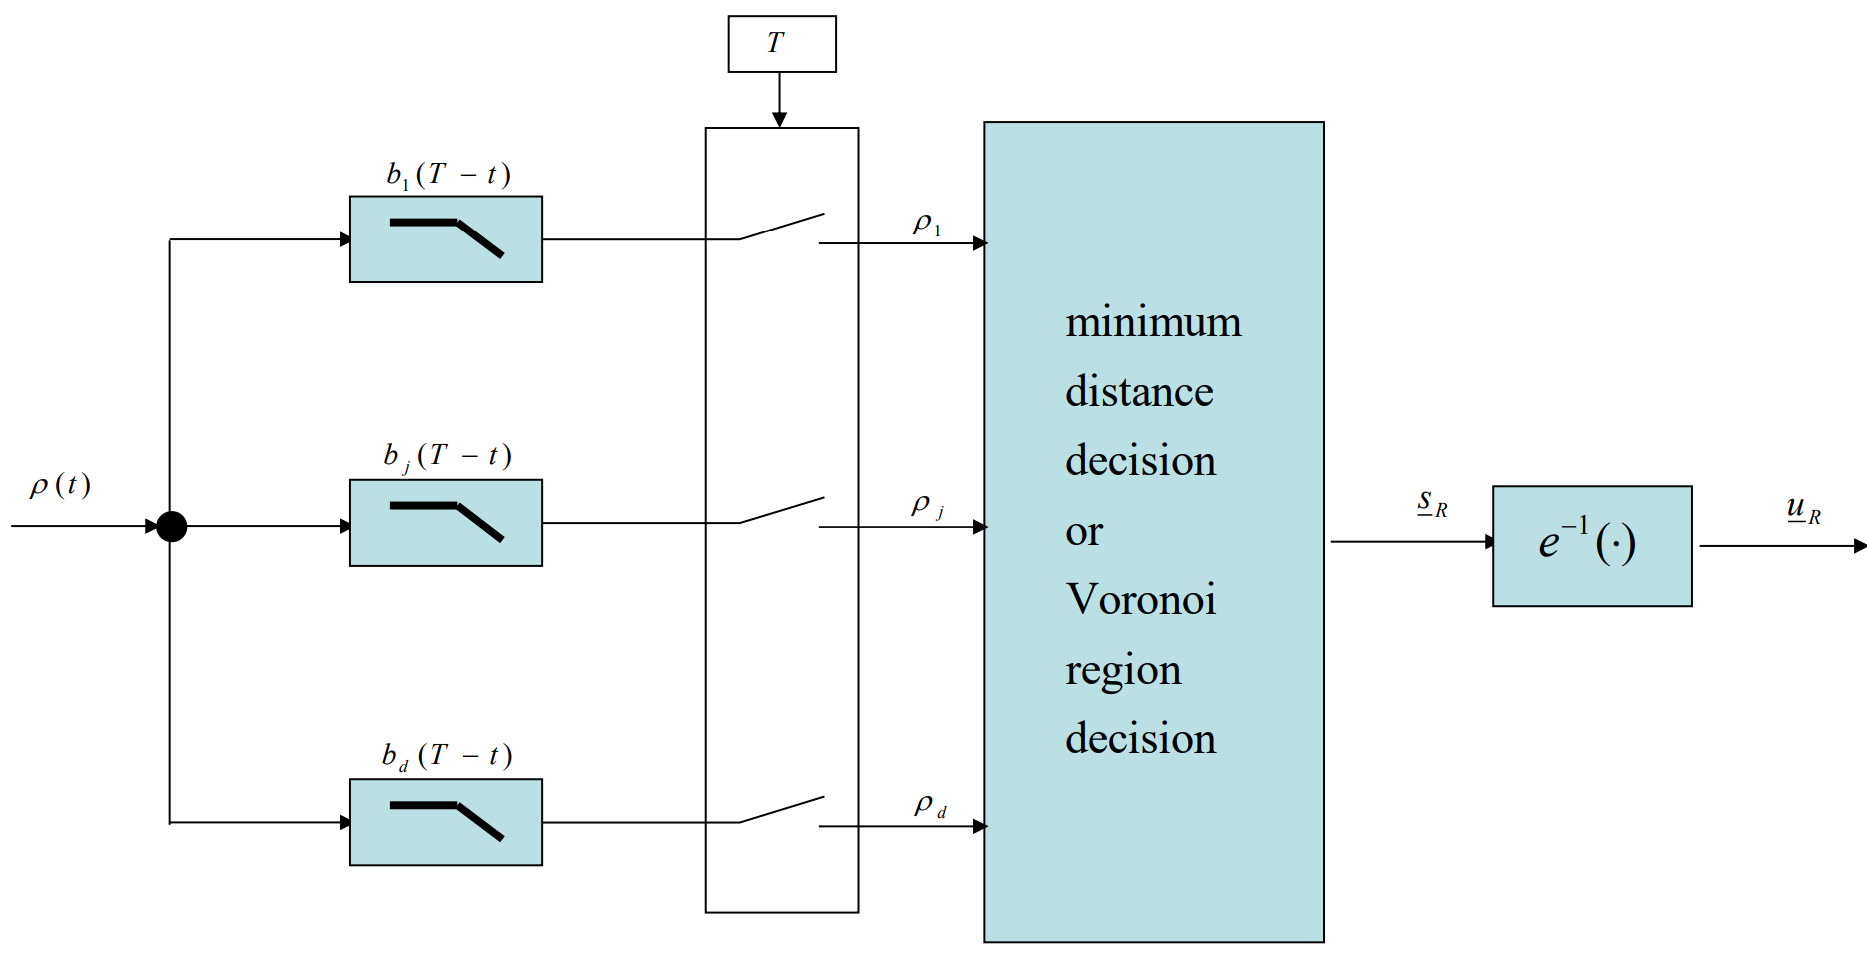
\includegraphics[width=\textwidth]{Img/MF.png}
    \end{center}
    \end{figure}
\end{center}
\newpage
\subsection{Giải thích Code}
Đầu tiên ta khai báo các thư viện để tính toán và mô phỏng các tín hiệu:
\begin{lstlisting}
import random
import numpy as np
import matplotlib.pyplot as plt
import math
\end{lstlisting}
Số lượng bit truyền đi: 8
Thời gian truyền 1 bit: 1
Thời gian truyền tín hiệu: 8
Tạo mạng bit ngẫu nhiên:
\begin{lstlisting}
N = 8      
Tb = 1     
T = 1*N    
t = np.arange(0, Tb, Tb/800)
def random_bits_array(n): 
    return [random.randint(0, 1) for _ in range(n)]
m = random_bits_array(N)
\end{lstlisting}
\textbf{Điều chế 2-ASK} \\
Chuyển các bit thành các tín hiệu tương ứng: \\ 
\begin{itemize}
    \item 1: $A_{1}sin(2\pi f t)$
    \item 0: $A_{2}sin(2\pi ft)$
\end{itemize}
Ta chọn $A_{1} = 1$ , $A_{2} = 0.25$ , $f = 2R_{b}$
\begin{lstlisting}
f = 2    
A1 = 1    
A2 = 0.25 
def modulation():
    out = []
    f = 2    
    A1 = 1    
    A2 = 0.25 
    t = np.arange(0, Tb, Tb/100)
    s1 = A1 * np.sin(2 * np.pi * f * t)
    s2 = A2 * np.sin(2 * np.pi * f * t)
    for i in range(len(m)):
        if m[i] == 0:
            out.extend(s2)
        if m[i] == 1:
            out.extend(s1)
    return out
ask = modulation()
\end{lstlisting}
Kết quả:\\
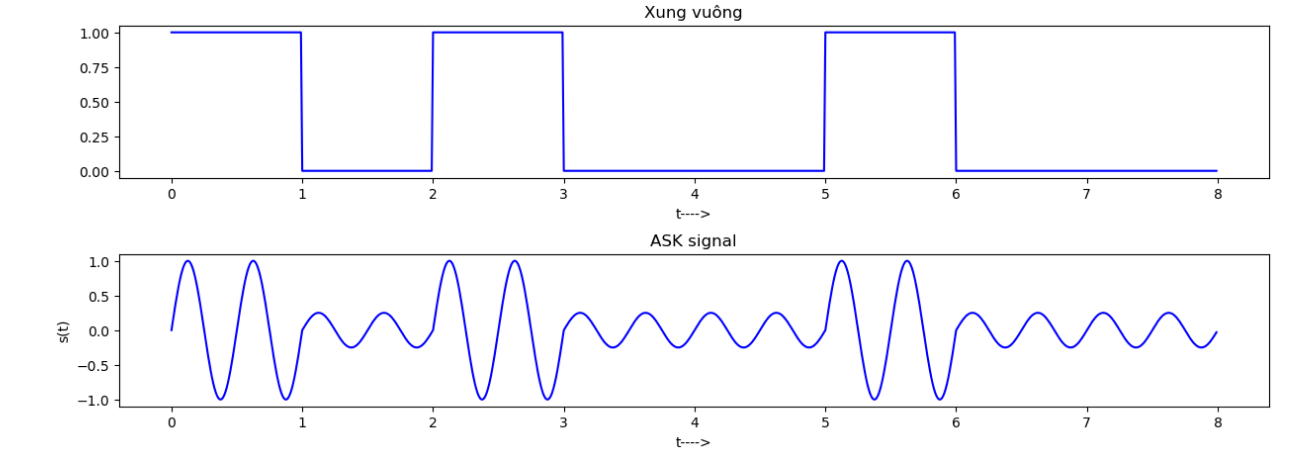
\includegraphics[width=\textwidth]{Img/ASK_f.png}
\\
\textbf{Thêm nhiễu Gauss} \\ 
Nhiễu Gauss được thêm vào có giá trị trung bình là 0, phương sai $\frac{N_{0}}{2}$
\begin{lstlisting}
N0 = 0.1
noise = np.random.normal(0, np.sqrt(N0/2), len(ask)) 
ask_noisy = ask + noise
\end{lstlisting}
Kết quả: \\
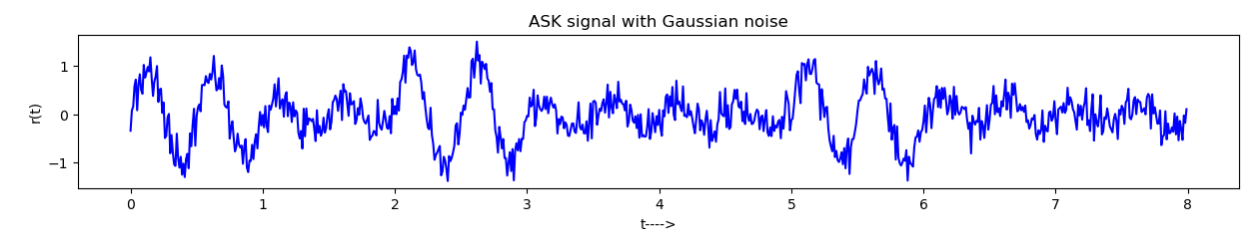
\includegraphics[width=\textwidth]{Img/ASK_N.png}
\textbf{Giải điều chế tín hiệu}\\
Cách làm: Ta tính hình chiếu của tín hiệu $r(t)$ trên cơ sơ trực chuẩn $B$ , sau đó ra quyết định bằng tiêu chuẩn khoảng cách ngắn nhất để khôi phục tín hiệu $s(t)$ ở nơi nhận. \\
Cơ sở trực chuẩn $B = \{b(t) = \sqrt{\frac{2}{T_{b}}}sin(2\pi ft)\}$\\
Sử dụng bộ lọc phối hợp tính các hình chiếu của $r(t)$ lên không gian trực chuẩn $M$:\\
$\rho[n] = \int_{nT_{b}}^{(n+1)T_{b}} \rho(t)b_{j}(t)\  dt $ \\
Áp dụng tiêu chuẩn khoảng cách nhỏ nhất ta suy ra:\\
Nếu $\rho[n] \geq \sqrt{\frac{T_{b}}{2}}\frac{(A_{1}+A_{2})}{2} $, ký tự nhị phân khôi phục $s'[n] = 1$.\\
Nếu $\rho[n] < \sqrt{\frac{T_{b}}{2}}\frac{(A_{1}+A_{2})}{2} $, ký tự nhị phân khôi phục $s'[n] = 0$.\\
Source code:
\begin{lstlisting}
def demodulation():
    t = np.arange(0, Tb, Tb/100)
    hx = math.sqrt(2/Tb)*np.sin(2 * np.pi * f * t)
    ask_noisy_list = np.array_split(ask_noisy, 8)
    output = []
    for i in range(len(ask_noisy_list)):
        if np.trapz(ask_noisy_list[i] * hx,t) >= np.sqrt(Tb
/2)*(A1+A2)/2:
            output.append(1)
        else:
            output.append(0)
    return output

demod = demodulation()
\end{lstlisting}
Kết quả: \\
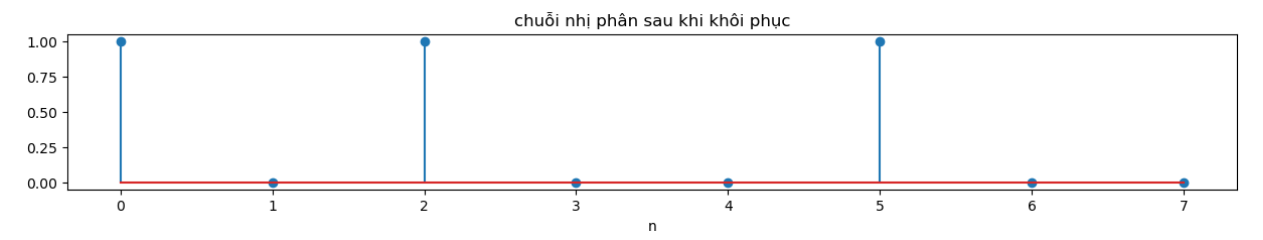
\includegraphics[width=\textwidth]{Img/In_Signal.png}
\subsection{Xác xuất lỗi:}
Ta đã có kết luận: Các không gian tín hiệu khác nhau (khác dạng sóng truyền) nhưng có cùng không gian vector thì có BER như nhau.\\
Do đó $BER = SER = \frac{1}{2}erfc(\sqrt{\frac{E_{0}}{N_{0}}})$
